\clearpage

\section{仿真对比}

第三章和第四章分别给出了等待 ALOHA 与等待 CSMA 的系统模型、稳态接入分析以及平均 AoI 和 AoI 违规概率的闭式表达式。理论推导能够揭示性能变化的内在机理，但这些表达式是否能够准确刻画有限规模网络中的实际行为，仍然需要通过进行数值仿真来做进一步的验证。与此同时，所提等待机制的实际价值也不能只停留在解析层面，还需要与已有的相关协议进行横向比较。

基于上述考虑，本章在统一的仿真框架下，先对等待 ALOHA 和等待 CSMA 的理论表达式进行验证，再分别与多种随机接入协议进行性能上的横向对比。本章内容安排如下：5.1 节介绍仿真设置与对比对象；5.2 节分别验证等待 ALOHA 和等待 CSMA 理论表达式的准确性，并结合仿真结果给出性能洞察；5.3 节将所提机制与已有 ALOHA 类和 CSMA 类协议进行横向比较；5.4 节对本章工作进行总结。

\subsection{仿真设置}

本章采用蒙特卡洛方法对系统进行仿真，来分别得到平均 AoI 与 AoI 违规概率的结果，用来与仿真结果进行对比的理论曲线分别由第三章和第四章得到的闭式表达式直接计算获得，其中等待 ALOHA 的理论结果分别对应式\eqref{cp3_AoI_Final}与式\eqref{cp3_violation_prob_simplified}，等待 CSMA 的理论结果分别对应式\eqref{cp4_AoI_Final}与式\eqref{cp4_violation_prob_simplified}。在同一组实验中，除图中横轴所对应的变量外，其余参数均保持不变。

为便于比较，本章将实验分为两类。第一类用于验证理论表达式的准确性，分别考察节点数量 $N$ 和等待窗口 $z$ 变化时理论值与仿真值的一致程度；第二类用于比较不同机制在同一负载条件下的性能表现。ALOHA 类机制的对比对象包括经典时隙 ALOHA 和文献\cite{yavascan2021analysis}提出的阈值 ALOHA；CSMA 类机制的对比对象包括标准 CSMA、文献\cite{maatouk2020age}提出的睡眠 CSMA，以及文献\cite{tripathi2023fresh}提出的 Fresh CSMA。节点规模的验证图主要用来观察网络负载提高后理论模型是否仍能贴合仿真结果，等待窗口的验证图则关注等待窗口的变化对 AoI 性能的影响。

\subsection{理论表达式验证}

\subsubsection{等待 ALOHA}

图\ref{fig:cp5_aloha_n_validation}给出了固定等待窗口 $z=60$ 时，等待 ALOHA 在节点数量变化条件下的理论值与仿真值对比结果。图\ref{fig:cp5_aloha_n_validation_aoi}与图\ref{fig:cp5_aloha_n_validation_violation}分别对应平均 AoI 和 AoI 违规概率的结果。

\begin{figure}[htbp]
    \centering
    \subfigure[平均 AoI 随节点数量变化\label{fig:cp5_aloha_n_validation_aoi}]{
        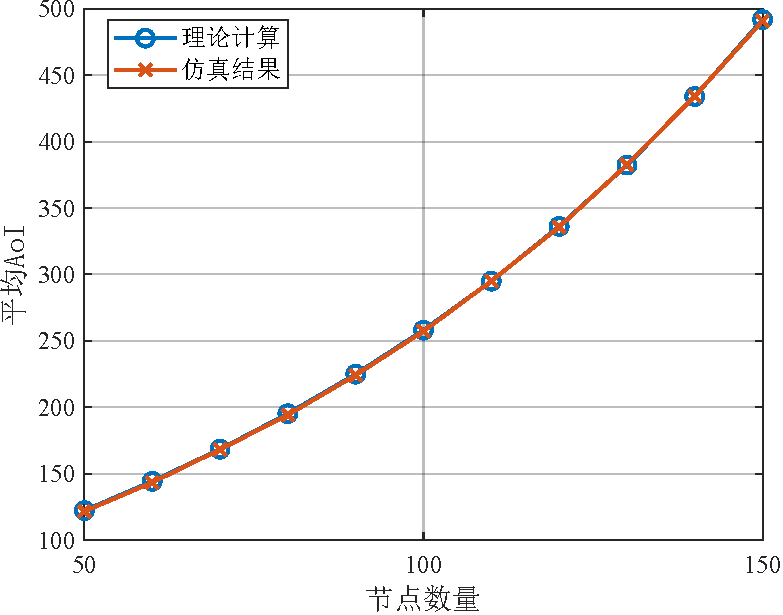
\includegraphics[width=0.47\textwidth]{figure/cp5/aloha/AoI_N50150z60.pdf}
    }
    \hfill
    \subfigure[AoI 违规概率随节点数量变化\label{fig:cp5_aloha_n_validation_violation}]{
        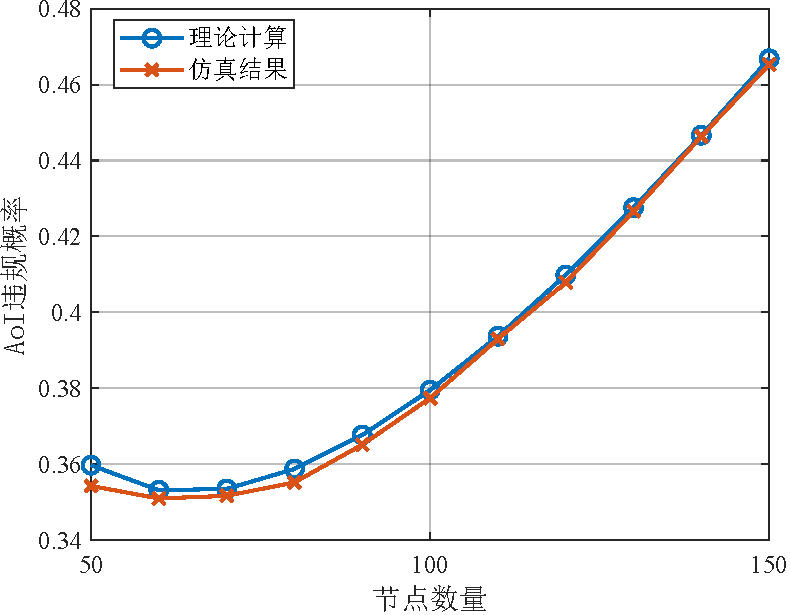
\includegraphics[width=0.47\textwidth]{figure/cp5/aloha/Violation_N50150z60.pdf}
    }
    \caption{固定等待窗口 $z=60$ 时等待 ALOHA 的理论与仿真对比}
    \label{fig:cp5_aloha_n_validation}
\end{figure}

从图\ref{fig:cp5_aloha_n_validation}可以看出，无论是平均 AoI 还是 AoI 违规概率，理论计算结果与仿真结果都保持了良好的一致性，说明第三章基于解耦假设、马尔可夫链建模以及矩匹配近似得到的闭式表达式能够较准确地刻画系统的稳态行为。随着节点数量的增加，碰撞概率也随之增大，离开时间间隔 $Y$ 的均值和方差都会增大，因此这两个指标整体呈恶化趋势。

图\ref{fig:cp5_aloha_z_validation}给出了固定节点数量 $N=50$ 时，等待窗口变化条件下的理论值与仿真值对比结果。图\ref{fig:cp5_aloha_z_validation_aoi}和图\ref{fig:cp5_aloha_z_validation_violation}分别对应平均 AoI 与 AoI 违规概率的结果。

\begin{figure}[htbp]
    \centering
    \subfigure[平均 AoI 随等待窗口变化\label{fig:cp5_aloha_z_validation_aoi}]{
        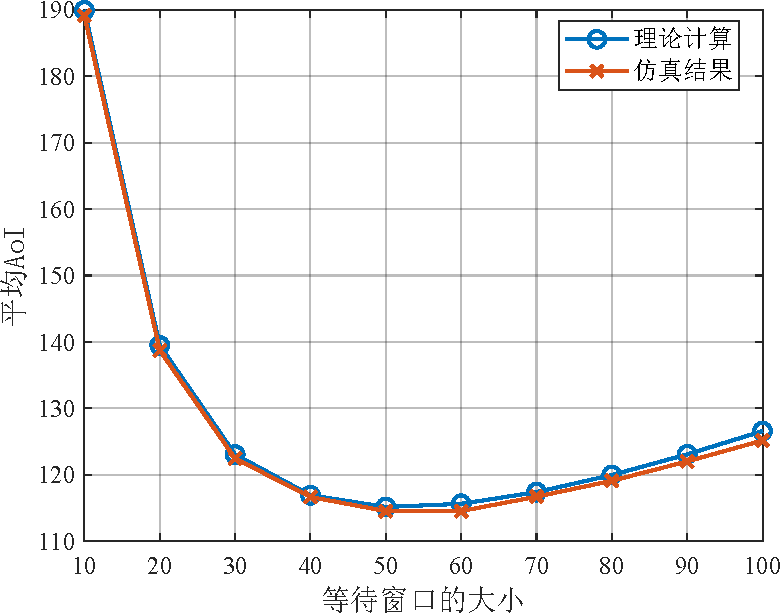
\includegraphics[width=0.47\textwidth]{figure/cp5/aloha/AoI_N50z10100.pdf}
    }
    \hfill
    \subfigure[AoI 违规概率随等待窗口变化\label{fig:cp5_aloha_z_validation_violation}]{
        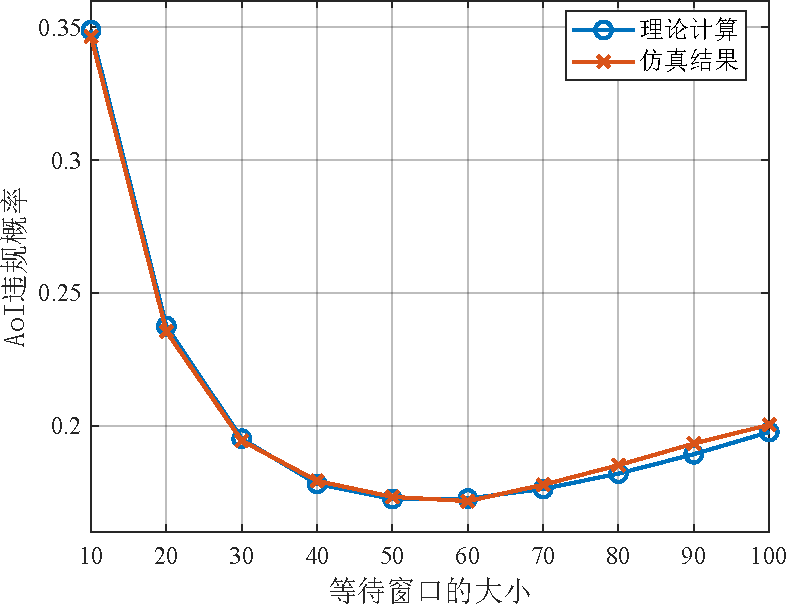
\includegraphics[width=0.47\textwidth]{figure/cp5/aloha/violation_N50z10100.pdf}
    }
    \caption{固定节点数量 $N=50$ 时等待 ALOHA 的理论与仿真对比}
    \label{fig:cp5_aloha_z_validation}
\end{figure}

从图\ref{fig:cp5_aloha_z_validation}的结果可以发现，当 $z$ 较小时，刚完成更新的节点会过早地回到信道竞争中来，无法有效地起到降低碰撞概率的作用，因此表现出来的性能相对较差；随着 $z$ 的增大，节点在完成更新后主动退避更长的时间，相当于直接减少了单位时隙内的活跃节点数量，因此性能得到了改善；随着 $z$ 的继续增大，虽然竞争强度进一步下降了，但成功更新后的确定性等待时间也在同步上升，过大的等待窗口会反过来拉长离开时间间隔，导致性能反而降低。因此，平均 AoI 与 AoI 违规概率都不会随着 $z$ 单调变化，而是会随着 $z$ 的增大呈现先减小后增加的变化规律。

\subsubsection{等待 CSMA}

图\ref{fig:cp5_csma_n_validation}给出了固定等待窗口 $z=64$ 时，等待 CSMA 在节点数量变化条件下的理论值与仿真值对比结果。图\ref{fig:cp5_csma_n_validation_aoi}与图\ref{fig:cp5_csma_n_validation_violation}分别对应平均 AoI 和 AoI 违规概率的结果。

\begin{figure}[htbp]
    \centering
    \subfigure[平均 AoI 随节点数量变化\label{fig:cp5_csma_n_validation_aoi}]{
        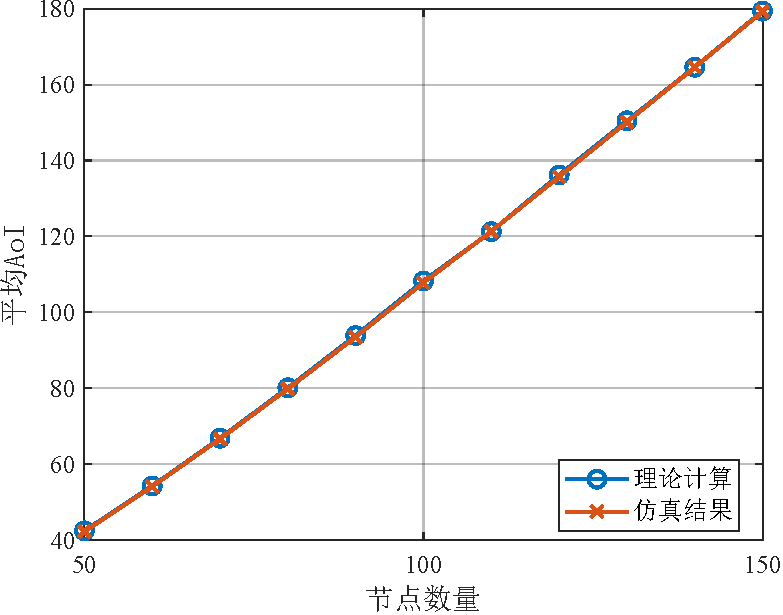
\includegraphics[width=0.47\textwidth]{figure/cp5/csma/AoI_N50150z64.pdf}
    }
    \hfill
    \subfigure[AoI 违规概率随节点数量变化\label{fig:cp5_csma_n_validation_violation}]{
        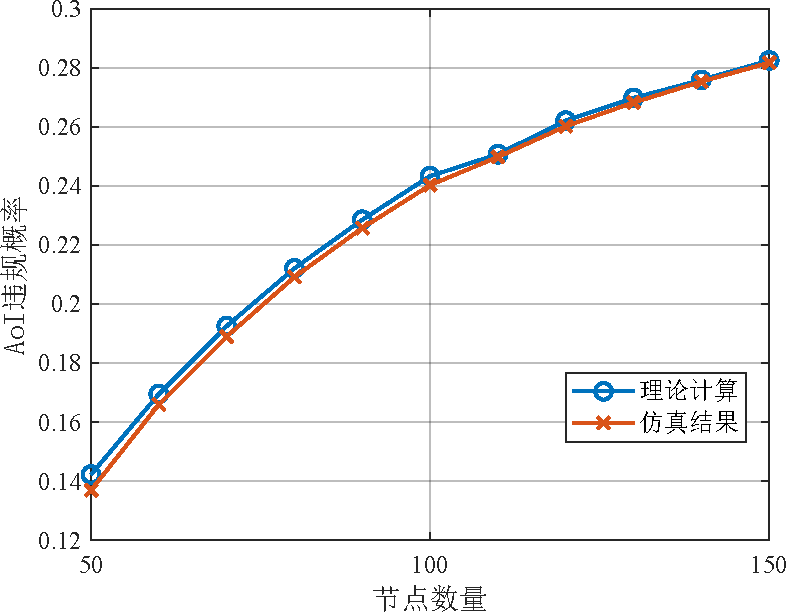
\includegraphics[width=0.47\textwidth]{figure/cp5/csma/violation_N50150z64.pdf}
    }
    \caption{固定等待窗口 $z=64$ 时等待 CSMA 的理论与仿真对比}
    \label{fig:cp5_csma_n_validation}
\end{figure}

从图\ref{fig:cp5_csma_n_validation}可以看出，第四章得到的理论表达式同样能够较准确地拟合等待 CSMA 的仿真结果。虽然载波侦听可以减少盲目碰撞发生的概率，但是随着节点数量的增加，系统中的忙碌时隙占比会逐步提高，竞争阶段和冻结阶段所带来的等待时间也会增加，因此平均 AoI 和 AoI 违规概率整体上仍表现为上升趋势。

图\ref{fig:cp5_csma_z_validation}给出了固定节点数量 $N=100$ 时，等待窗口变化条件下的理论值与仿真值对比结果。图\ref{fig:cp5_csma_z_validation_aoi}和图\ref{fig:cp5_csma_z_validation_violation}分别对应平均 AoI 与 AoI 违规概率的结果。

\begin{figure}[htbp]
    \centering
    \subfigure[平均 AoI 随等待窗口变化\label{fig:cp5_csma_z_validation_aoi}]{
        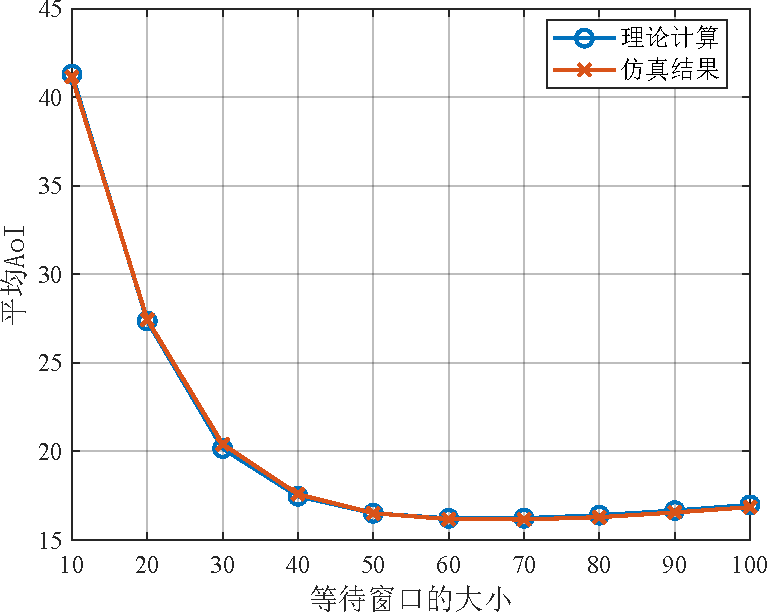
\includegraphics[width=0.47\textwidth]{figure/cp5/csma/AoI_N20z10100.pdf}
    }
    \hfill
    \subfigure[AoI 违规概率随等待窗口变化\label{fig:cp5_csma_z_validation_violation}]{
        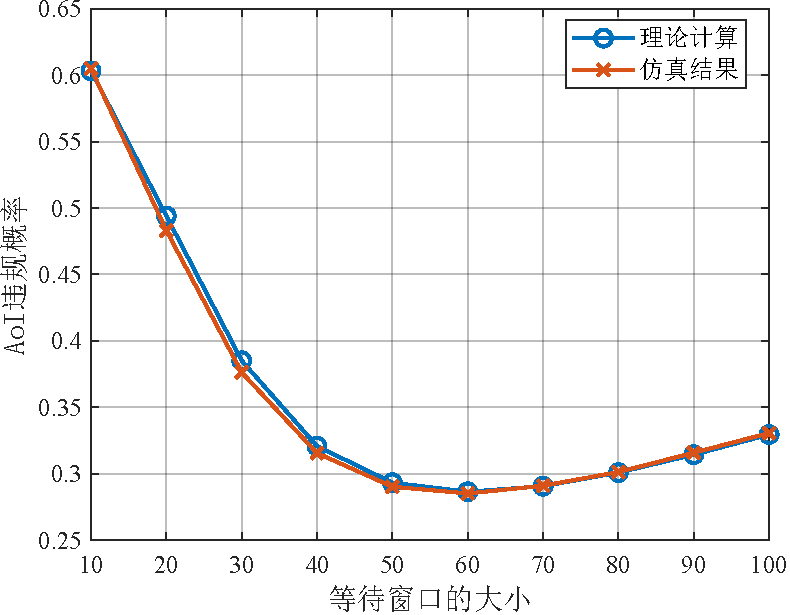
\includegraphics[width=0.47\textwidth]{figure/cp5/csma/violation_N20z10100.pdf}
    }
    \caption{固定节点数量 $N=20$ 时等待 CSMA 的理论与仿真对比}
    \label{fig:cp5_csma_z_validation}
\end{figure}

从图\ref{fig:cp5_csma_z_validation}的结果可以发现，等待 CSMA 下的平均 AoI 与 AoI 违规概率随等待窗口 $z$ 的变化规律与等待 ALOHA 类似。当 $z$ 过小时，刚完成更新的节点会过早地回到信道竞争中来，无法有效地起到降低碰撞概率的作用，因此表现出来的性能相对较差；随着 $z$ 的增大，节点在完成更新后会等待更长的时间，相当于直接减少了单位时隙内的活跃节点数量，因此性能得到了改善；随着 $z$ 的进一步增大，由于成功更新后的确定性等待时间过高，导致性能反而下降了。

\subsection{不同机制的性能对比}

\subsubsection{ALOHA 类机制对比}

图\ref{fig:cp5_aloha_comparison}给出了等待 ALOHA、经典时隙 ALOHA 以及阈值 ALOHA 在不同节点规模下的性能对比结果。图\ref{fig:cp5_aloha_comparison_aoi}与图\ref{fig:cp5_aloha_comparison_violation}分别对应平均 AoI与违规概率的对比结果。

\begin{figure}[htbp]
    \centering
    \subfigure[平均 AoI 对比\label{fig:cp5_aloha_comparison_aoi}]{
        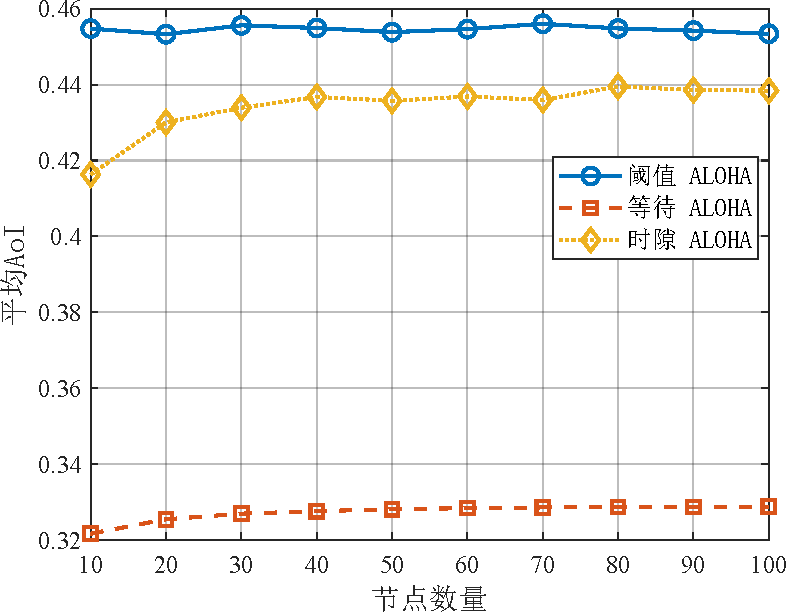
\includegraphics[width=0.47\textwidth]{figure/cp5/aloha/aoi_aloha.pdf}
    }
    \hfill
    \subfigure[AoI 违规概率对比\label{fig:cp5_aloha_comparison_violation}]{
        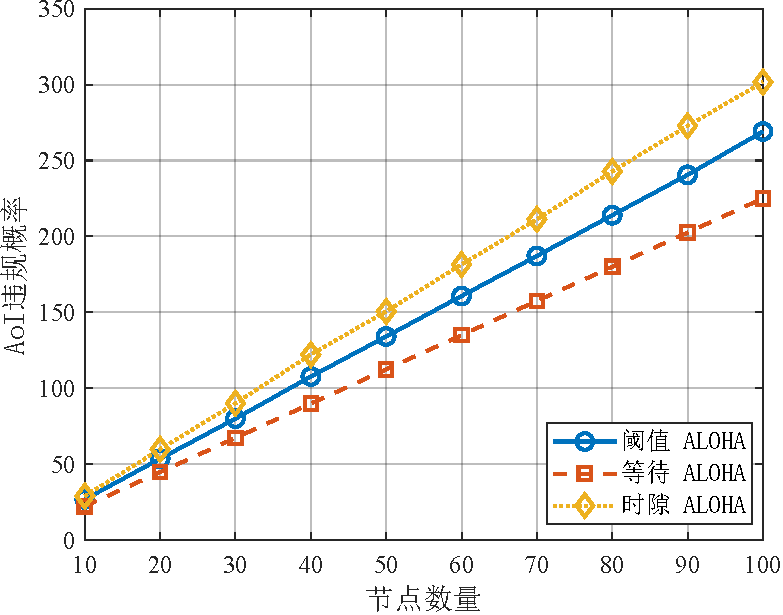
\includegraphics[width=0.47\textwidth]{figure/cp5/aloha/violation_aloha.pdf}
    }
    \caption{ALOHA 类机制的性能对比}
    \label{fig:cp5_aloha_comparison}
\end{figure}

从图\ref{fig:cp5_aloha_comparison}可以看出，等待 ALOHA 在所考察的规模范围内整体优于经典时隙 ALOHA 与阈值 ALOHA。经典时隙 ALOHA 不区分节点状态的新鲜程度，刚完成更新的节点仍会立即重新参与竞争，因此节点数量增加后更容易形成较高的碰撞强度，平均 AoI 与违规概率都会快速恶化。阈值 ALOHA 是通过年龄阈值压缩活跃节点的数量，以此来减少单位时隙内的活跃节点数量，从而来降低网络中的碰撞概率。这一策略在网络负载较轻的条件下是有效的，但当网络的负载上升后，碰撞概率急剧增加，大量节点由于无法成功传输而导致其在接收端的 AoI 不断增大，且由于该机制缺乏碰撞后的处理措施，导致它无法处理这种拥塞现象，随着时间的推移，所有节点的 AoI 都将突破原先设定的年龄阈值，阈值 ALOHA 将失去作用。

相比之下，等待 ALOHA 则通过对节点在成功传输后施加确定性等待，主动减少单位时隙内的活跃节点数量，以此来减少碰撞，并且保留了碰撞后的随机退避机制，保证了在高负载的条件下避免节点在碰撞后再次集中接入，由此确保了系统的稳定运行。

\subsubsection{CSMA 类机制对比}

图\ref{fig:cp5_csma_comparison}给出了等待 CSMA、标准 CSMA、睡眠 CSMA 以及 Fresh CSMA 的性能对比结果。图\ref{fig:cp5_csma_comparison_aoi}与图\ref{fig:cp5_csma_comparison_violation}分别对应平均 AoI 与违规概率的对比结果。

\begin{figure}[htbp]
    \centering
    \subfigure[平均 AoI 对比\label{fig:cp5_csma_comparison_aoi}]{
        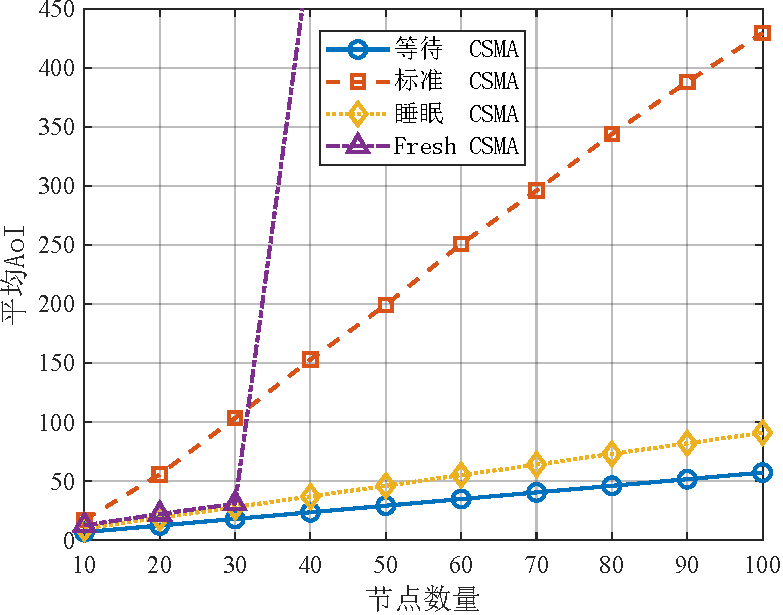
\includegraphics[width=0.47\textwidth]{figure/cp5/csma/aoi_csma.pdf}
    }
    \hfill
    \subfigure[AoI 违规概率对比\label{fig:cp5_csma_comparison_violation}]{
        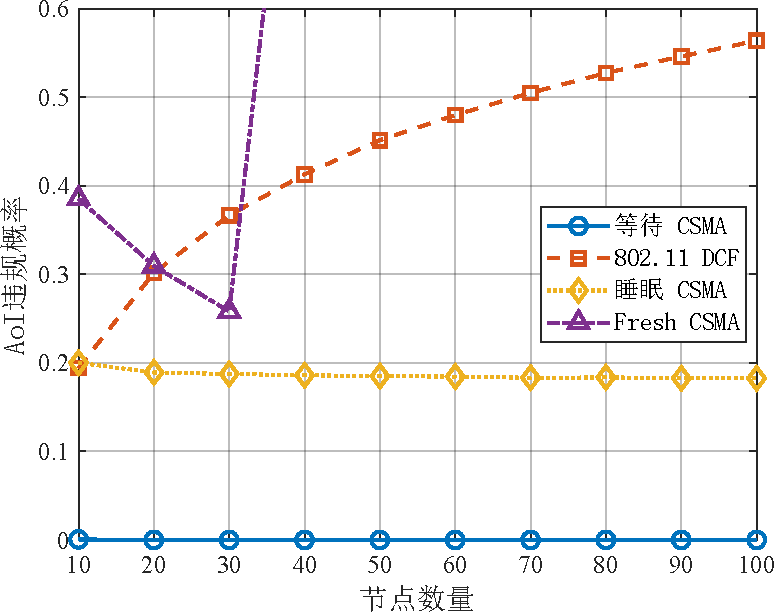
\includegraphics[width=0.47\textwidth]{figure/cp5/csma/violation_csma.pdf}
    }
    \caption{CSMA 类机制的性能对比}
    \label{fig:cp5_csma_comparison}
\end{figure}

从图\ref{fig:cp5_csma_comparison}可以看出，将等待机制引入标准 CSMA 后，系统在平均 AoI 和 AoI 违规概率两个指标上均有明显改善。标准 CSMA 的设计目标更偏向吞吐量和长期接入公平性，并不会主动限制刚完成更新节点的再次竞争，因此在 AoI 视角下并不占优。睡眠 CSMA 通过成功后的休眠来让出信道资源，较标准 CSMA 有所改进，但其等待时间由一个指数分布的随机数决定，容易得到一个较短的休眠时间，导致节点迅速地回到信道的竞争中来。Fresh CSMA 在理想化的条件下通过当前时刻的 AoI 来选择最优的退避计时器。但当节点数量过多时，由于无休止的碰撞，绝大部分甚至全部节点都处于较高的 AoI，根据 Fresh CSMA 的设计，节点将选择极短的退避计时器，甚至是0，这非但无法缓解碰撞的现象，反而会进一步加剧碰撞，由此导致 Fresh CSMA 在节点数量增加后 AoI 性能急剧恶化。相比之下，等待 CSMA 在建立系统模型时便将信道的碰撞因素考虑在内，因此在存在碰撞的真实环境下，等待 CSMA 依旧能展现出良好的性能。

综合图\ref{fig:cp5_aloha_comparison}与图\ref{fig:cp5_csma_comparison}可以看出，等待随机接入机制并不依赖某一种特定的底层 MAC 框架。无论是在等长时隙的 ALOHA 环境中，还是在具备载波侦听和变长系统时隙的 CSMA 环境中，适度限制成功节点的再次接入，并对碰撞后的节点进行处理，都是改善 AoI 性能的有效思路。

\subsection{本章小结}

本章围绕等待 ALOHA 与等待 CSMA 的理论表达式验证和横向性能对比展开。首先，通过节点数量变化和等待窗口变化两类实验，验证了第三章与第四章所推导的平均 AoI 和 AoI 违规概率表达式的准确性，说明基于马尔可夫链、解耦近似以及矩匹配建立的分析框架能够较稳定地刻画系统稳态性能。在此基础上，本章进一步将所提机制与现有的随机接入协议进行了对比。结果表明，无论在 ALOHA 场景还是 CSMA 场景下，等待机制都能够在平均 AoI 与 AoI 违规概率两个指标上取得更优越的表现。尤其是在网络规模增大、竞争更为激烈时，这种优势更加明显。
